\documentclass[11pt]{exam}
\usepackage[utf8]{inputenc}
\usepackage[a4paper,top=2cm,left=2cm,right=2cm,bottom=2cm]{geometry}
\usepackage{import}
\usepackage[T1]{fontenc}
\usepackage[german,ngerman]{babel}
\usepackage[table]{xcolor}
\usepackage{amsthm, esvect}
\usepackage{mathtools}
\RequirePackage{amssymb, amsfonts, amsmath, latexsym, verbatim, xspace}
\usepackage{systeme}
\usepackage{multicol}
\usepackage{multirow}
\usepackage{framed}
\usepackage{array}
\usepackage{ragged2e}
\usepackage{graphicx}
\usepackage{pdflscape}
\usepackage{epstopdf}
\usepackage{booktabs}
\usepackage{pdfpages}
\usepackage{float} % Allows putting an [H] in \begin{figure} to specify the exact location of the figure
\usepackage{wrapfig} % Allows in-line images such as the example fish picture
\usepackage{tikz, graphicx} % tikz
\usepackage[position=top]{subfig}
\usepackage[bookmarks=true]{hyperref}%Links
\usepackage{enumerate}
\usepackage{enumitem}
\usepackage[german,ruled,vlined,linesnumbered,algosection]{algorithm2e}
\usepackage[labelfont=sf]{caption}
\usepackage{lmodern}
\usepackage{lscape}
\usepackage{tabularx}
\usepackage{systeme}
\usepackage{hhline}
\usepackage{subfiles}
\usepackage{stackengine}
\usepackage{setspace}
\usepackage{MnSymbol}
\usepackage{tcolorbox}
\usepackage{bbm}
\usepackage{url}
\usepackage{xparse}
\usepackage{sectsty}
\usepackage{array}
\usepackage{ragged2e}
\usepackage{listings} %Stellt Code-Snippets sauber dar

% definiert die Sprache
\selectlanguage{German}

% add command for different dates in Swiss fashion
\newcommand{\monthwordlong}[1]{\ifcase#1 \or Januar\or Februar\or März\or April\or Mai\or Juni\or Juli\or August\or September\or Oktober\or November\or Dezember\fi}
\newcommand{\monthwordshort}[1]{\ifcase#1\or Jan\or Feb\or Mar\or Apr\or Mai\or Jun\or Jul\or Aug\or Sept\or Okt\or Nov\or Dez\fi}
\newcommand{\datelong}{\number\day.\:\monthwordlong{\the\month}\:\number\year}
\newcommand{\dateshort}{\number\day.\:\monthwordshort{\the\month}\:\number\year}

% define color of links inside a text
\definecolor{linkblue}{RGB}{0, 0, 80}
\definecolor{plotblue}{RGB}{100, 100, 255}
\definecolor{myblue}{RGB}{8,164,214}
\definecolor{myred}{RGB}{143,42,41}
\definecolor{forestgreen}{RGB}{34,139,34}
\definecolor{highdive}{RGB}{10,169,194}
\definecolor{charcoal}{RGB}{74,74,74}
\hypersetup{
	colorlinks=true,
	linkcolor=linkblue,
	filecolor=magenta,
	urlcolor=plotblue,
	citecolor=linkblue,
	pdfpagemode=FullScreen,
}


\lstdefinestyle{mystyle}{ % definiert den style des Code-Snippets
	%backgroundcolor=\color{backcolour},
	%commentstyle=\color{codegreen},
	%keywordstyle=\color{magenta},
	%numberstyle=\tiny\color{codegray},
	%stringstyle=\color{codepurple},
	basicstyle=\ttfamily\footnotesize,
	breakatwhitespace=false,
	breaklines=true,
	captionpos=b,
	keepspaces=true,
	%numbers=left,
	%numbersep=5pt,
	showspaces=false,
	showstringspaces=false,
	showtabs=false,
	tabsize=4
}
\lstset{style=mystyle}
\qformat{\Large\textbf{Aufgabe \thequestion\hfill\thepoints}}
\newlist{partes}{enumerate}{3}
\setlist[partes]{label=(\alph*)}
\newcommand{\parte}{\item}
\newlist{subpartes}{enumerate}{3}
\setlist[subpartes]{label=\roman*)}
\newcommand{\subparte}{\item}
\setlist[enumerate,1]{%(
	leftmargin=*, itemsep=12pt, label={\textbf{\arabic*.)}}}
\newcommand\answerbox{%%
	\fbox{\rule{2in}{0pt}\rule[-0.1ex]{0pt}{4ex}}}
\pointpoints{Punkt}{Punkte}
\hqword{Frage:}
\hpword{Mögliche Punkte:}
\hsword{Erreicht:}
\htword{Total}
\renewcommand*\half{.5}
\renewcommand{\solutiontitle}{\noindent\textbf{Lösung:}\par\noindent}

% Graphed boxes
\newcommand{\karos}[2]{
  \begin{tikzpicture}
    \draw[step=0.4cm,color=cyan,dotted] (0,0) grid (#1 cm ,#2 cm);
  %  \draw((#1)/2 cm,0)--((#1)/2 cm,/#2)/2cm)
  \end{tikzpicture}
}
\usetikzlibrary{arrows, petri, topaths, graphs}
\linespread{1.2} % Line spacing

%=========================================================
\newenvironment{parcols}[1][]{
    \begin{parts}\begin{multicols}{#1}
}{
    \end{multicols}\end{parts}
}
%=========================================================
\newenvironment{itemcols}[1][]{
	\begin{itemize}\begin{multicols}{#1}
		}{
	\end{multicols}\end{itemize}
}

%=========================================================
\newcommand{\antwort}[1]{
	{\setlength{\textwidth}{\textwidth}\fillwithgrid{#1cm}\vspace{5pt}}
}

%=========================================================
% Karriertes Papier für Antwort MIT OVERLAY
\tcbuselibrary{breakable,skins}
\usetikzlibrary{mindmap,trees}
\newlength\tindent
\setlength{\tindent}{\parindent}
\setlength{\parindent}{0pt}
\setlength{\parskip}{0pt}

\newtcolorbox{gridspace}[1]{%
	enhanced,
	breakable,
	blanker,
	boxrule=0pt,
	left=5mm,
	right=5mm,
	top=5.75mm,
	bottom=0mm,
	boxsep=0pt,
	height=#1cm,
	width=16cm,
	before upper={
		\begingroup
		\setlength{\baselineskip}{5.75mm}
		\setlength{\parskip}{0pt}
		\setlength{\lineskip}{0pt}
		% keep every paragraph on the grid rhythm
		%\everypar{\vspace{0pt}\strut}
		% math formulas shifted by one grid row
		\let\oldbracketopen\[
		\renewcommand{\[}{\vspace{-5mm}\oldbracketopen}
		% Align displayed formulas to the grid
		\setlength{\abovedisplayskip}{0pt}
		\setlength{\belowdisplayskip}{0pt}
		\setlength{\abovedisplayshortskip}{0pt}
		\setlength{\belowdisplayshortskip}{0pt}
		% Enumerate follows the same rhythm
		\setlist[enumerate]{leftmargin=6mm,itemsep=0mm,topsep=0pt,parsep=0pt,partopsep=0pt}
		\setlist[itemize]{leftmargin=6mm,itemsep=10mm,topsep=0pt,parsep=0pt,partopsep=0pt}},
	after upper={
		\endgroup},
	underlay={
		\draw[step=5mm,color=gray!55] (interior.south west) grid (interior.north east);}
}

\pagestyle{headandfoot}
\firstpageheader{}{}{\teacher}
\runningheader{}{}{\teacher}
\firstpagefooter{}{}{Seite \thepage\:von \numpages}
\runningfooter{}{}{Seite \thepage\:von \numpages}
%%
% Math Arrows
%%
\newcommand{\same}{\ensuremath{\Longleftrightarrow}}
\renewcommand{\to}{\ensuremath{\longrightarrow}}
\newcommand{\qsame}{\quad\same\quad}
\newcommand{\dsame}{\ensuremath{:\Leftrightarrow}}
\newcommand{\qdsame}{\quad\dsame\quad}
\newcommand{\ldsame}{\ensuremath{:\Longleftrightarrow}}
\newcommand{\samedef}{\ensuremath{\us {\text{def}} \Leftrightarrow}}
\newcommand{\qsamedef}{\quad\samedef\quad}
\newcommand{\lsamedef}{\ensuremath{\us {\text{def}} \Longleftrightarrow}}
\newcommand{\qlsamedef}{\quad\lsamedef\quad}


%%
% Mengendefinitionen
%%
\newcommand{\M}{\ensuremath{\mathcal{M}}}
\newcommand{\N}{\ensuremath{\mathbb{N}}}
\newcommand{\Z}{\ensuremath{\mathbb{Z}}}
\newcommand{\Q}{\ensuremath{\mathbb{Q}}}
\newcommand{\I}{\ensuremath{\mathbb{I}}}
\newcommand{\R}{\ensuremath{\mathbb{R}}}
\newcommand{\C}{\ensuremath{\mathbb{C}}}
\renewcommand{\S}{\ensuremath{\mathbb{S}}}
\newcommand{\Prim}{\ensuremath{\mathbb{P}}}
\newcommand{\0}{\ensuremath{\emptyset}}
\renewcommand{\Re}{\ensuremath{\operatorname{Re}}}
\renewcommand{\Im}{\ensuremath{\operatorname{Im}}}
\newcommand{\strich}{\ensuremath{\big\vert}}

%%
% Mengenoperation
%%
\renewcommand{\nin}{\not\in}


%%
% Logisches Und und Oder
%%
\newcommand{\sand}{\ensuremath{\; \land \;}}
\newcommand{\sor}{\ensuremath{\; \lor \;}}
\renewcommand{\*}{\ensuremath{\cdot}}
\newcommand{\oder}{\vee}
\newcommand{\n}{\neg}
\newcommand{\und}{\wedge}


%%
% Bei Integral, Summe,... die Grenzen über bzw.
% unter das Zeichen
%%
\renewcommand{\d}[1]{\ensuremath{\operatorname{d}\!{#1}}}
\newcommand{\Sum}{\sum\limits}
\newcommand{\Prod}{\prod\limits}
\newcommand{\Min}{\min\limits}
\newcommand{\Max}{\max\limits}
\newcommand{\Lim}{\lim\limits}
\newcommand{\Inf}{\inf\limits}
\newcommand{\Sup}{\sup\limits}
\newcommand{\Liminf}{\liminf\limits}
\newcommand{\Limsup}{\limsup\limits}
%\renewcommand{\Cup}{\bigcup\limits}
%\renewcommand{\Cap}{\bigcap\limits}
\newcommand{\Otimes}{\bigotimes\limits}
\newcommand{\Oplus}{\bigoplus\limits}


%%
% Arcus Cotangens, Logarithmus
%%
\let\oldsin\sin
\renewcommand{\sin}[1]{\oldsin{\left(#1\right)}}
\let\oldcos\cos
\renewcommand{\cos}[1]{\oldcos{\left(#1\right)}}
\let\oldtan\tan
\renewcommand{\tan}[1]{\oldtan{\left(#1\right)}}
\let\oldarcsin\arcsin
\renewcommand{\arcsin}[1]{\oldarcsin{\left(#1\right)}}
\let\oldarccos\arccos
\renewcommand{\arccos}[1]{\oldarccos{\left(#1\right)}}
\let\oldarctan\arctan
\renewcommand{\arctan}[1]{\oldarctan{\left(#1\right)}}
\let\oldln\ln
\renewcommand{\ln}[1]{\oldln{\left(#1\right)}}
\newcommand{\Log}[2]{\ensuremath{\operatorname{log}_{#1}\left(#2\right)}}
\newcommand{\e}{\operatorname{e}}
\renewcommand{\exp}[1]{\ensuremath{\operatorname{\e}^{#1}}}


%%
% Griechische Buchstaben
%%
\renewcommand{\epsilon}{\ensuremath{\varepsilon}}
\renewcommand{\phi}{\varphi}
\renewcommand{\l}{\lambda}
\renewcommand{\t}{\tau}


%%
% Bezeichnungen
%%
\newcommand{\Rgn}{\R_{>0}} % R grösser Null
\newcommand{\Rad}{\operatorname{Rad}}   % Radikal
\newcommand{\kgV}{\operatorname{kgV}}   % Kleinster gemeinsame Vielfache
\newcommand{\ggT}{\operatorname{ggT}}   % Grösster gemeinsame Teiler
\newcommand{\winkel}{\sphericalangle}          % Winkelsymbol
\DeclarePairedDelimiter\abs{\lvert}{\rvert} % besserer Betrag
\makeatletter
\let\oldabs\abs
\def\abs{\@ifstar{\oldabs}{\oldabs*}}
\makeatother


%%
% Vektorgeometrie
%%
\renewcommand{\v}[1]{\vv{#1}}       % besserer Pfeil über Buchstaben
\renewcommand{\vec}[2]{\begingroup\renewcommand{\arraystretch}{1}\left(\begin{array}{c} #1 \\ #2 \end{array}\right)\endgroup}   % two dimensional vector
\renewcommand{\Vec}[3]{\begingroup\renewcommand{\arraystretch}{1}\left(\begin{array}{c} #1 \\ #2 \\ #3 \end{array}\right)\endgroup}      % three dimensional vector


%%
% Text
%%
\newcommand*{\Ueq}[1]{\mathrel{\mathop{=}\limits_{\text{#1}}}}
\newcommand*{\Oeq}[1]{\mathrel{\stackrel{\text{#1}}{=}}}
\newcommand{\utext}[2]{\underbrace{#1}_{\substack{#2}}}
\newcommand{\otext}[2]{$\overbrace{\textrm{#1}}^{\textrm{#2}}$}
\newcommand{\lineortext}[1]{\hspace{0,1cm}\underline{\hspace{0.1cm}\hphantom{#1}\hspace{0.1cm}}\hspace{0,1cm}} % Lückentext erstellen
\newcommand{\gap}[1]{\rule{#1 cm}{1pt}}
%=========================================================
\newcommand{\theme}{Strahlensätze}
\newcommand{\teacher}{Jonas Guler}
%=========================================================
\begin{document}
\fontsize{14}{14}\selectfont
\begin{center}
    \huge\bf\theme
\end{center}

\begin{questions}
%=========================================================
%-------------------TESTFRAGEN
%=========================================================
\noaddpoints
\question[\totalpoints]
\addpoints
Formuliere je einen 1. und einen 2. Strahlensatz aus der folgenden Figur (als Formeln).\newline
\begin{minipage}{0.35\linewidth}
    \centering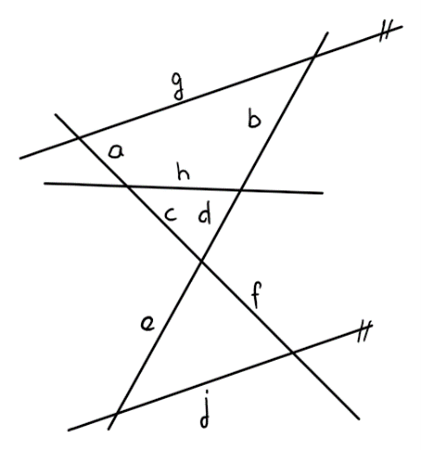
\includegraphics[scale=1]{data-geometrie/strahlensatzfigurkomplex.png}
\end{minipage}
\hfill
\begin{minipage}{0.6\linewidth}
    \begin{parts}
        \part[1] 1. Strahlensatz\vspace{2cm}
        \part[1] 2. Strahlensatz\vspace{2cm}
    \end{parts}
\end{minipage}

%---------------------------------------------------------
\question[4]
Bestimme die unbekannten Seiten $a,b,c,d$ in der Figur unten.
\begin{figure}[H]
    \centering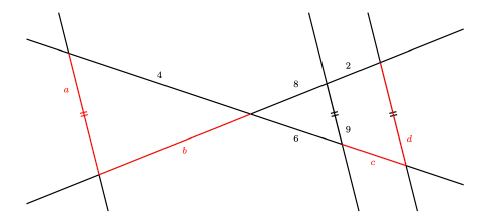
\includegraphics[scale=0.8]{data-geometrie/strahlensatz2.png}
\end{figure}

%---------------------------------------------------------
\question[4]
Bestimme die unbekannten Seiten $a,b,c,d$ in der Figur unten.
\begin{figure}[H]
    \centering\includegraphics[scale=0.8]{data-geometrie/strahlensatz3.png}
\end{figure}

%---------------------------------------------------------
\question[4]
Berechne die Länge der unbekannten Strecken $w,x,y$ und $z$.
\begin{figure}[H]
	\centering
\includegraphics[width=0.5\linewidth]{strahlensatz4.png}
\end{figure}

%---------------------------------------------------------
\question[4]
Berechne die Länge der unbekannten Strecken $w,x,y$ und $z$.
\begin{figure}[H]
	\centering
\includegraphics[width=0.45\linewidth]{strahlensatz5.png}
\end{figure}

%---------------------------------------------------------
\question[5]
Begründe mit Hilfe der Strahlensätze, ob alle drei, nur zwei oder keine der Geraden $a,b,c$ parallel sind.
\begin{figure}[H]
    \centering
\includegraphics[width=0.4\linewidth]{parallelität_wahr.png}
\end{figure}

%---------------------------------------------------------
\question[4]
Begründe mit Hilfe der Strahlensätze, ob alle drei, nur zwei oder keine der Geraden $a,b,c$ parallel sind.
\begin{figure}[H]
    \centering
\includegraphics[width=0.4\linewidth]{parallelität_falsch.jpeg}
\end{figure}

%---------------------------------------------------------
\question[3]
\begin{minipage}{0.45\linewidth}
	Unter einer Treppe soll ein $78$cm breiter Schrank eingebaut werden. Wie hoch kann der Schrank maximal sein?
\end{minipage}
\hfill
\begin{minipage}{0.53\linewidth}
	\centering
\includegraphics[scale=0.4]{schrankuntertreppe.png}
\end{minipage}


%---------------------------------------------------------
\question[5]
Für ein Flugzeug soll ein neuer Hangar gebaut werden. Die Masse des Hangars sind rechts im Querschnitt angegeben. Vom Tor weiss man, dass es $50$m breit ist. Leider ist im Plan die Höhe vergessen gegangen. Berechne sie.
\begin{figure}[H]
    \centering
\includegraphics[scale=0.1]{flugzeughangar.png}
\end{figure}

%---------------------------------------------------------
\question[5]
Frau Kurz (Augenhöhe $1.7$m) bestimmt die Höhe einer Tanne. Von ihrem Balkon aus peilt sie über einen Telefonmast die Tannenspitze an. In der Zeichnung unten sind die gemessenen Stecken und Längen eingezeichnet. Wie hoch ist die Tanne?
\begin{figure}[H]
	\centering
\includegraphics[width=0.5\linewidth]{baumhöhe.png}
\end{figure}

%---------------------------------------------------------
\question[4]
\begin{minipage}{0.55\linewidth}
    Betrachte die nebenstehende Figur (Skizze!). Entscheide, ob die beiden Dreiecke $\triangle ABC$ und $\triangle ADE$ zueinander ähnlich sind. Begründe deine Antwort.
\end{minipage}
\hfill
\begin{minipage}{0.4\linewidth}
    \centering
\includegraphics[scale=0.8]{ähnlicheDreiecke.jpg}
\end{minipage}

%---------------------------------------------------------
\question[4]
\begin{minipage}{0.6\linewidth}
    $ABCD$ und $EBFG$ sind zwei Rechtecke. Entscheide und begründe, welche der vier Dreiecke ähnlich sind.
\end{minipage}
\hfill
\begin{minipage}{0.35\linewidth}
    \centering
\includegraphics[scale=0.8]{RechteckeMitÄhnlichkeit.png}
\end{minipage}

%---------------------------------------------------------
\question[5]
\begin{minipage}{0.65\linewidth}
    Von der nebenstehenden Figur wissen wir, dass $\overline{BC}$ parallel zu $\overline{DE}$ und $\overline{CD}$ parallel zu $\overline{EF}$ sind. Weiter sind $\overline{AF}=4$ und $\overline{DF}=3$ lang. Wie lang ist die Strecke $\overline{BD}$?
\end{minipage}
\hfill
\begin{minipage}{0.3\linewidth}
    \centering
\includegraphics[scale=0.5]{doppelterstrahlensatz.png}
\end{minipage}

%---------------------------------------------------------
\question[4]
Gegeben ist ein gleichschenkliges Dreieck $\triangle ABC$ mit Höhe $h_a=36$cm und Basis $a=12$cm. Das einbeschriebene Rechteck $DEFG$ hat einen Umfang von $30$cm. Berechne die Länge und Breite des Rechtecks.
\begin{figure}[H]
    \centering
\includegraphics[scale=0.8]{rechteckstrahlensatz.png}
\end{figure}


%---------------------------------------------------------
\question[3]
\begin{minipage}{0.6\linewidth}
    Die Fläche des kleineren Dreiecks beträgt $36\%$ des grösseren. Berechne $x$.
\end{minipage}
\hfill
\begin{minipage}{0.35\linewidth}
    \centering
\includegraphics[scale=0.4]{ähnlicheflächen.png}
\end{minipage}
\vspace{5pt}

%---------------------------------------------------------
\question[2]
Entscheide in der Tabelle unten, ob die Aussagen wahr oder falsch sind. Die Antworten müssen nicht begründet werden.\newline
\begin{small}
    Bewertung: Für $0-2$ korrekte Antworten gibt es keine Punkte; $3$ korrekte Antworten einen Punkt und falls alle Antworten korrekt sind, gibt es $2$ Punkte.
\end{small}
\begingroup
\renewcommand{\arraystretch}{1.5}
\begin{table}[H]
    \centering
    \begin{tabular}{|p{12cm}|c|c|}\hline
         & wahr & falsch \\\hline
        Zwei Rechtecke, bei denen eine Seite $3$cm lang ist, sind ähnlich. & & \\\hline
        Zwei Parallelogramme mit dem Seitenverhältnis 3:4 sind ähnlich. & & \\\hline
        Zwei gleichschenklige Dreiecke sind ähnlich. & & \\\hline
        Für negative Streckfaktoren sind die beiden Dreiecke nicht ähnlich. & & \\\hline
    \end{tabular}
\end{table}
\endgroup

\end{questions}
\end{document}